\section{Materials and methods}

\subsection{Selection of the RNA-seq data}

This study uses publicly available paired-end RNA-seq\index{RNA-seq!paired-end} data of wild and cultivated rice, submitted in January 1, 2021 by the Institute of Botany, Chinese Academy of Sciences. This data allows to compare rice grown under normal conditions with rice grown under drought stress conditions. Furthermore, the data allows for an interspecies comparison of wild rice (Oryza nivara\index{Oryza!nivara}, cultivars BJ278\index{cultivar!BJ278} and BJ89\index{cultivar!BJ89}) with cultivated rice (Oryza sativa\index{Oryza!sativa}, cultivar Nipponbare\index{cultivar!Nipponbare}).

All samples were uniformly taken from seedlings (leaf tissue) at the age of twelve days. Used sequencing platform: Illumina HiSeq 2000\index{Illumina!HiSeq 2000}.

All this makes the data well suited for a targeted analysis of drought stress responses.


\subsection{Quality evaluation}

The quality of the raw and trimmed RNA-seq data\index{RNA-seq!quality assessment} was assessed using FastQC\index{FastQC} \autocite{babraham}. FastQC is a quality control analysis tool for high throughput sequencing data. It provides information about
\begin{itemize}
    \item \emph{basic statistics}: some simple composition statistics for the FASTQ\index{FASTQ} file analyzed
    \item \emph{per base sequence quality}: an overview of the range of quality values across all bases at each position in the FASTQ file
    \item \emph{per tile sequence quality}: an overview of the per tile sequence quality in case an Illumina library was used
    \item \emph{per sequence quality scores}: an overview of how the overall quality scores of the sequences are distributed
    \item \emph{per base sequence content}: an overview of the proportion of each base position in a FASTQ file for which each of the four normal DNA bases has been called
    \item \emph{per sequence GC content}: the GC content across the whole length of each sequence in a file compared with a normal distributed GC content
    \item \emph{per base N content}: an overview of the N content at each position across all bases
    \item \emph{sequence length distribution}: an overview of how the sequence lengths are distributed
    \item \emph{sequence duplication levels}: an overview of the degree of duplication for every sequence in a library
    \item \emph{over-represented sequences}: a list of over-represented sequences matched against common contaminants\index{RNA-seq!contaminant}
    \item \emph{adapter content}: a check for significant amounts of adapter sequences\index{RNA-seq!adapter sequence} the FASTQ file
\end{itemize}

The results of the separate FastQC analyses (of the raw and trimmed FASTQ files), the results of the Trimmomatic\index{Trimmomatic} trimming and the information about the kallisto\index{kallisto} pseudoalignments\index{transcript!pseudoalignment} were summarized in an interactive MultiQC\index{MultiQC} HTML-report. See \autocite{10.1093/bioinformatics/btw354}.


\subsection{RNA-seq preprocessing}

The initial quality assessment of the raw FASTQ files revealed that about roughly the first 12 base pairs of the reads were of low quality. Therefore, the data was preprocessed/trimmed using Trimmomatic\index{Trimmomatic}, a "flexible and efficient preprocessing tool, which could correctly handle paired-end data" \autocite{10.1093/bioinformatics/btw354}.

That trimming substantially improved the per base sequence content and the per base sequence quality. Figures \ref{fig:0.1-FastQC-per_base_seq_cont-CRR240976-raw_vs_trim} and \ref{fig:0.1-FastQC-per_base_seq_qual-CRR240976-raw_vs_trim} show exemplary a comparison of the FastQC assessments of a raw FASTQ file vs the corresponding trimmed FASTQ file.

\begin{figure}[htbp]
    \caption[Exemplary FastQC quality assessment of the per base sequence content - raw vs trimmed FASTQ file]{FastQC quality assessment of the per base sequence content of the raw FASTQ file CRR240976\_f1.fastq.gz vs the trimmed file CRR240976\_f1.trim.p.fastq.gz}
    \label{fig:0.1-FastQC-per_base_seq_cont-CRR240976-raw_vs_trim}
    \begin{subfigure}[t]{0.48\linewidth}
        \caption{Raw data}
        \label{fig:0.1-FastQC-per_base_seq_cont-CRR240976}
        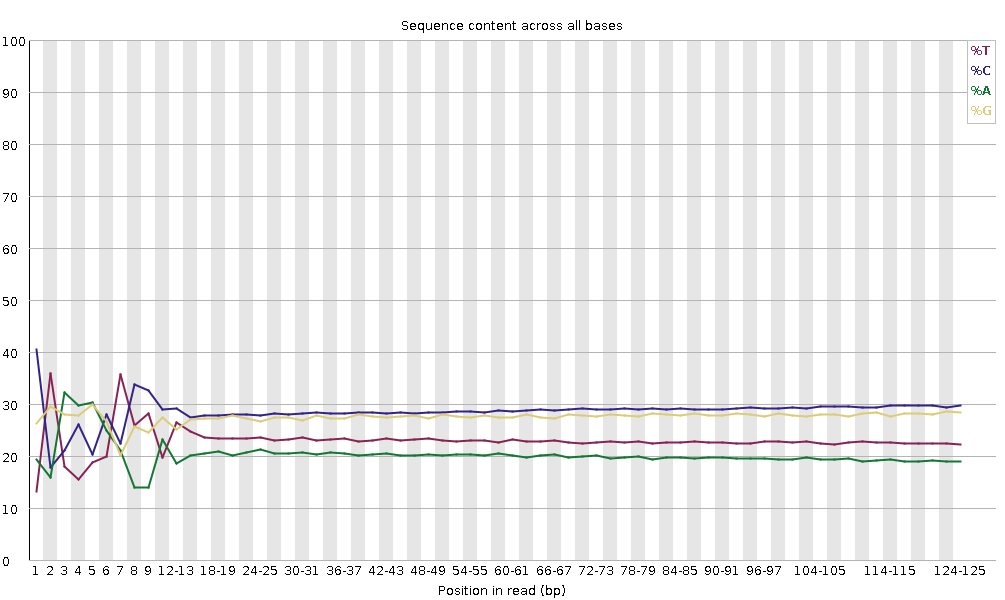
\includegraphics[width=\textwidth, height=4cm]{../../results/fastqc/Plot-Exports/fastqc_per_base_sequence_content_plot_CRR240976_f1}
    \end{subfigure}
    \begin{subfigure}[t]{0.48\linewidth}
        \caption{Trimmed data}
        \label{fig:0.1-FastQC-per_base_seq_cont-CRR240976-trim}
        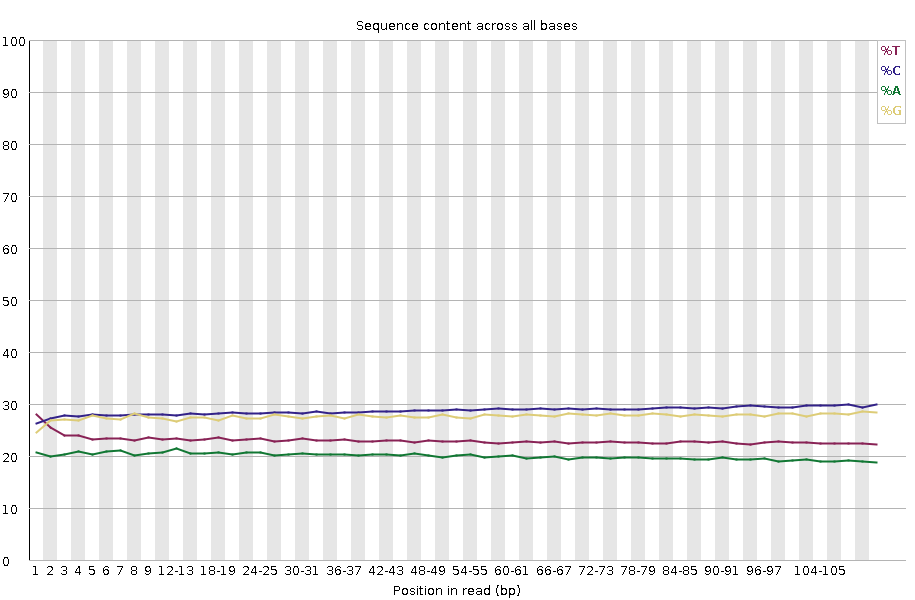
\includegraphics[width=\textwidth, height=4cm]{../../results/fastqc/Plot-Exports/fastqc_per_base_sequence_content_plot_CRR240976_f1_trim_p}
    \end{subfigure}
\end{figure}

\begin{figure}[htbp]
    \caption[Exemplary FastQC quality assessment of the per base sequence quality - raw vs trimmed FASTQ file]{FastQC quality assessment of the per base sequence quality of the raw FASTQ file CRR240976\_f1.fastq.gz vs the trimmed file CRR240976\_f1.trim.p.fastq.gz}
    \label{fig:0.1-FastQC-per_base_seq_qual-CRR240976-raw_vs_trim}
    \begin{subfigure}[t]{0.48\linewidth}
        \caption{Raw data}
        \label{fig:0.1-FastQC-per_base_seq_qual-CRR240976}
        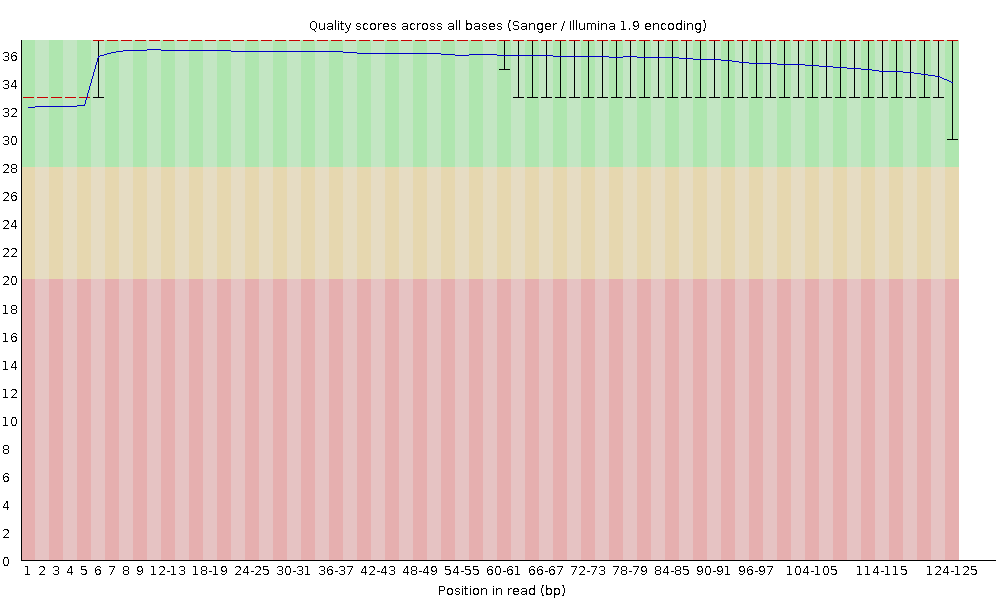
\includegraphics[width=\textwidth, height=4cm]{../../results/fastqc/Plot-Exports/fastqc_per_base_sequence_quality_plot_CRR240976_f1}
    \end{subfigure}
    \begin{subfigure}[t]{0.48\linewidth}
        \caption{Trimmed data}
        \label{fig:0.1-FastQC-per_base_seq_qual-CRR240976-trim}
        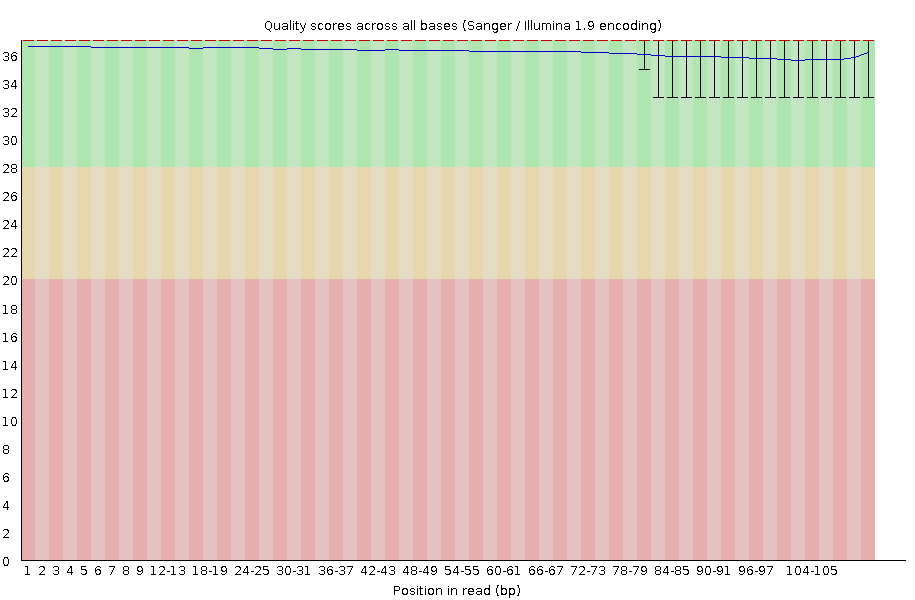
\includegraphics[width=\textwidth, height=4cm]{../../results/fastqc/Plot-Exports/fastqc_per_base_sequence_quality_plot_CRR240976_f1_trim_p}
    \end{subfigure}
\end{figure}


\subsection{Transcripts abundances quantification}

The mapping/pseudoalignment of the RNA-seq reads and the abundances quantification of the transcripts\index{transcript!abundances quantification} was done using kallisto\index{kallisto}. According to \autocite{10.1038/nbt.3519}, kallisto offers the following advantages over other alignment and quantification software:
\begin{quote}
    kallisto is a program for quantifying abundances of transcripts from RNA-Seq data, or more generally of target sequences using high-throughput sequencing reads. It is based on the novel idea of pseudoalignment for rapidly determining the compatibility of reads with targets, without the need for alignment. On benchmarks with standard RNA-Seq data, kallisto can quantify 30 million human bulk RNA-seq reads in less than 3 minutes on a Mac desktop computer using only the read sequences and a transcriptome index that itself takes than 10 minutes to build. Pseudoalignment of reads preserves the key information needed for quantification, and kallisto is therefore not only fast, but also comparably accurate to other existing quantification tools. In fact, because the pseudoalignment procedure is robust to errors in the reads, in many benchmarks kallisto significantly outperforms existing tools.
\end{quote}

kallisto requires a reference genome/transcriptome\index{genome/transcriptome!reference} for aligning the RNA-seq data. To this end, reference FASTA\index{FASTA} cDNA\index{DNA!cDNA} dumps of Oryza nivara, cultivar BJ278 and Oryza sativa, cultivar Nipponbare were downloaded from Ensembl\index{Ensembl}. The Ensembl project delivers reference data for genome interpretation for any species: genome assemblies from public archive are annotated with genes, regulatory regions, variants and comparative data to provide a foundation for scientific research and genome interpretation \autocite{10.1093/nar/gkab1049}.


\subsection{Statistical evaluation and differential expression analysis}

The preprocessed and aligned data was further evaluated and analyzed using an R-script\index{R} \autocite{R-base} executed within RStudio\index{R!RStudio} \autocite{RStudio}. The following sections describe the analysis steps in detail.

\subsubsection{Import of the kallisto transcript-level estimates}

The kallisto transcript-level estimates were imported using the R-package \verb|tximport|\index{R!package!tximport} \autocite{R-tximport, tximport2015}. Thereby, the  abundances, counts, and transcript lengths were summarized to the gene level.

Scaling method: average transcript length over samples and then the library size (parameter \verb|lengthScaledTPM|).

The mapping of the transcript IDs\index{transcript!ID} (used within the kallisto \verb|abundance.tsv| files) to the corresponding gene IDs\index{gene!ID} was done using the BioMart database \verb|plants_mart| hosted at \url{https://plants.ensembl.org}. Datasets: \verb|nivara_eg_gene| and \verb|osativa_eg_gene| for O. nivara and O. sativa, respectively. See \autocite{R-biomaRt, biomaRt2009}.

Figure \ref{fig:2.1-TPM-Stats} shows some basic transcripts per million (TPM\index{transcript!transcripts per million (TPM)}) statistics about the imported kallisto files.

\begin{figure}[htbp]
    \caption{TPM statistics about the imported kallisto data}
    \label{fig:2.1-TPM-Stats}
    \begin{subfigure}[t]{0.48\linewidth}
        \caption{O. nivara}
        \label{fig:2.1-TPM-Stats-Oryza_nivara}
        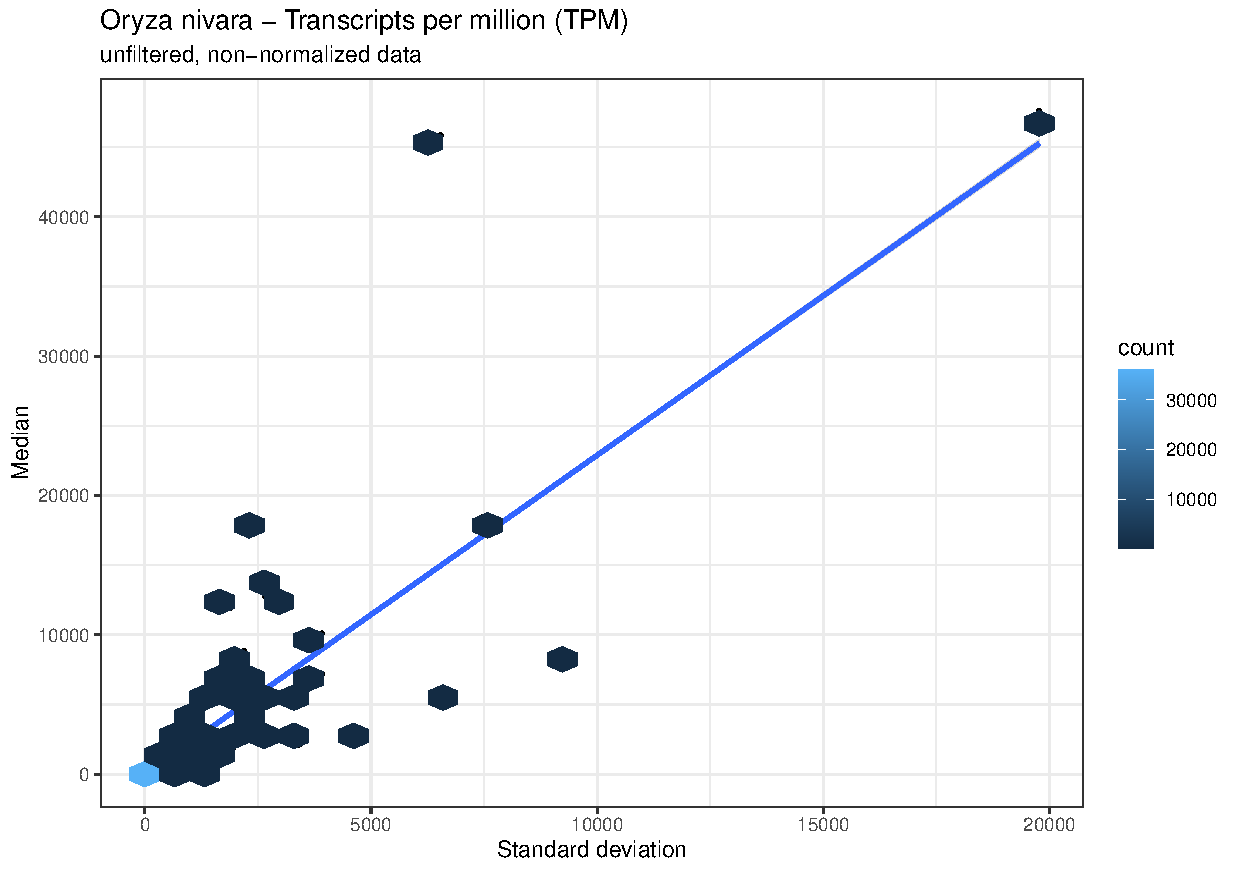
\includegraphics[width=\textwidth]{../../results/plots-and-tables/2.1-TPM-Stats-Oryza_nivara}
    \end{subfigure}
    \begin{subfigure}[t]{0.48\linewidth}
        \caption{O. sativa}
        \label{fig:2.1-TPM-Stats-Oryza_sativa}
        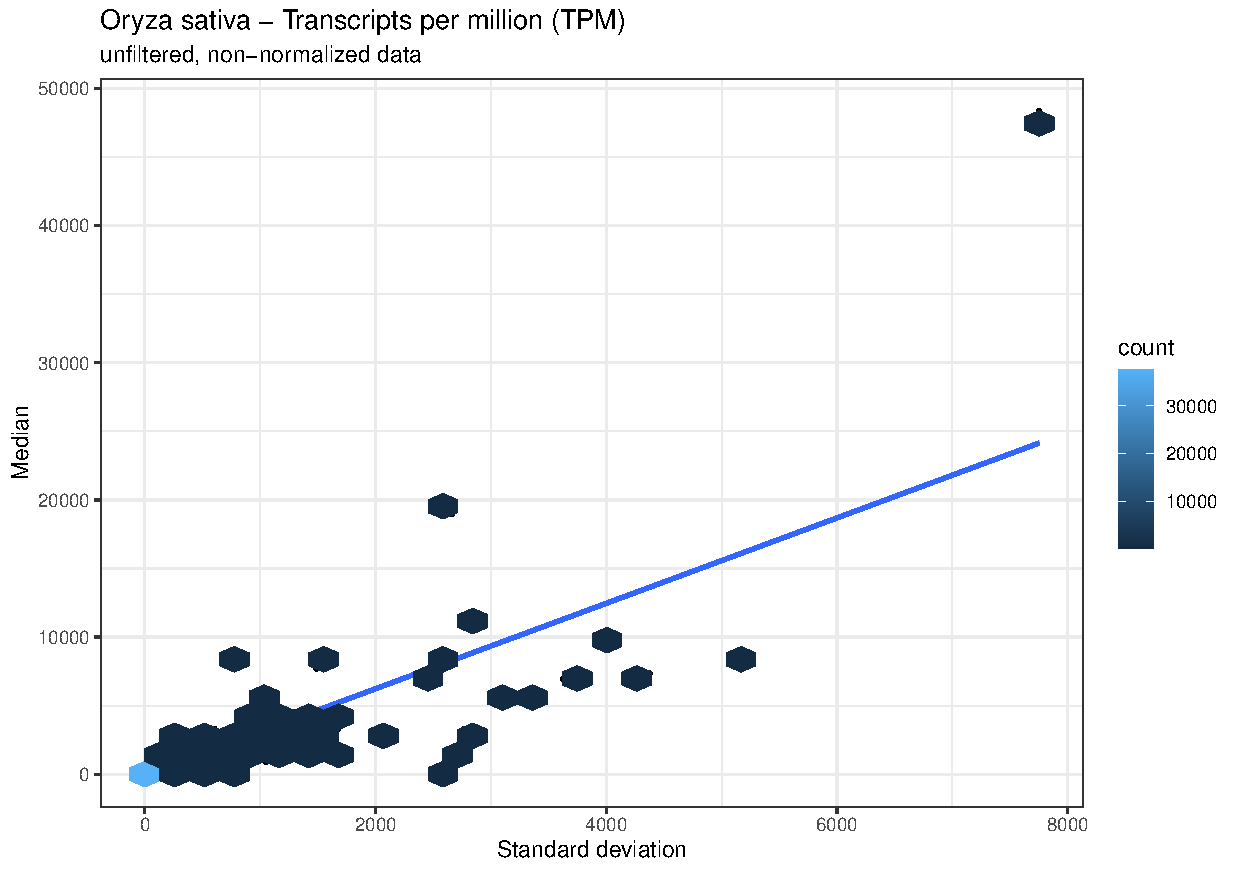
\includegraphics[width=\textwidth]{../../results/plots-and-tables/2.1-TPM-Stats-Oryza_sativa}
    \end{subfigure}
\end{figure}

\subsubsection{Filtering and normalization}

For further analysis, \verb|DGEList|-objects with counts per million (CPM)\index{counts per million (CPM)} and log2(CPM) values were created using the R-package \verb|edgeR|\index{R!package!edgeR} \autocite{R-edgeR, edgeR2010}. Figure \ref{fig:2.2-Log2CPM-unflt-notnorm} shows the distribution of the log2(CPM) values.

\begin{figure}[htbp]
    \caption{Log2(CPM) distribution of the unfiltered, non-normalized data}
    \label{fig:2.2-Log2CPM-unflt-notnorm}
    \begin{subfigure}[t]{0.64\linewidth}
        \caption{O. nivara}
        \label{fig:2.2-Log2CPM-unflt-notnorm-Oryza_nivara}
        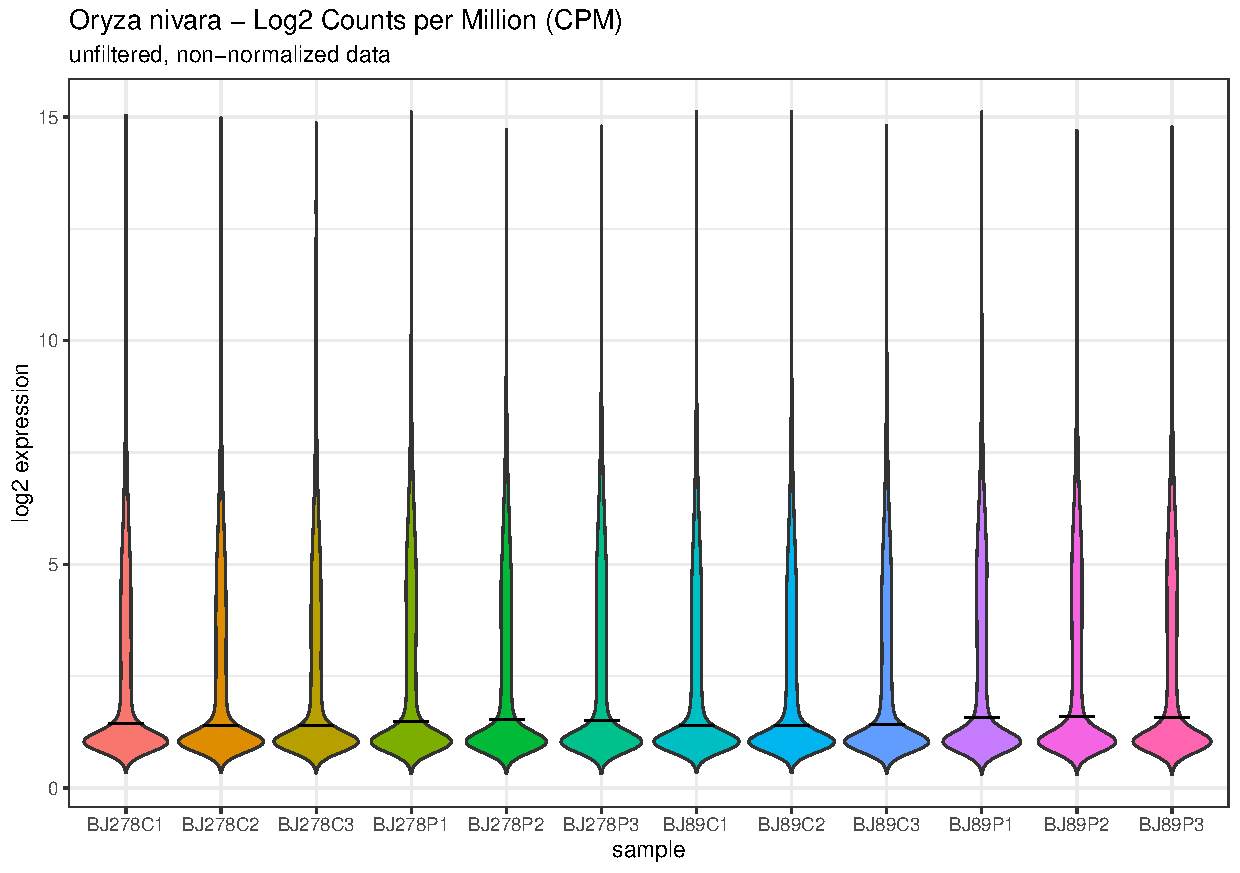
\includegraphics[width=\textwidth, height=3cm]{../../results/plots-and-tables/2.2-Log2CPM-unflt-notnorm-Oryza_nivara}
    \end{subfigure}
    \begin{subfigure}[t]{0.32\linewidth}
        \caption{O. sativa}
        \label{fig:2.2-Log2CPM-unflt-notnorm-Oryza_sativa}
        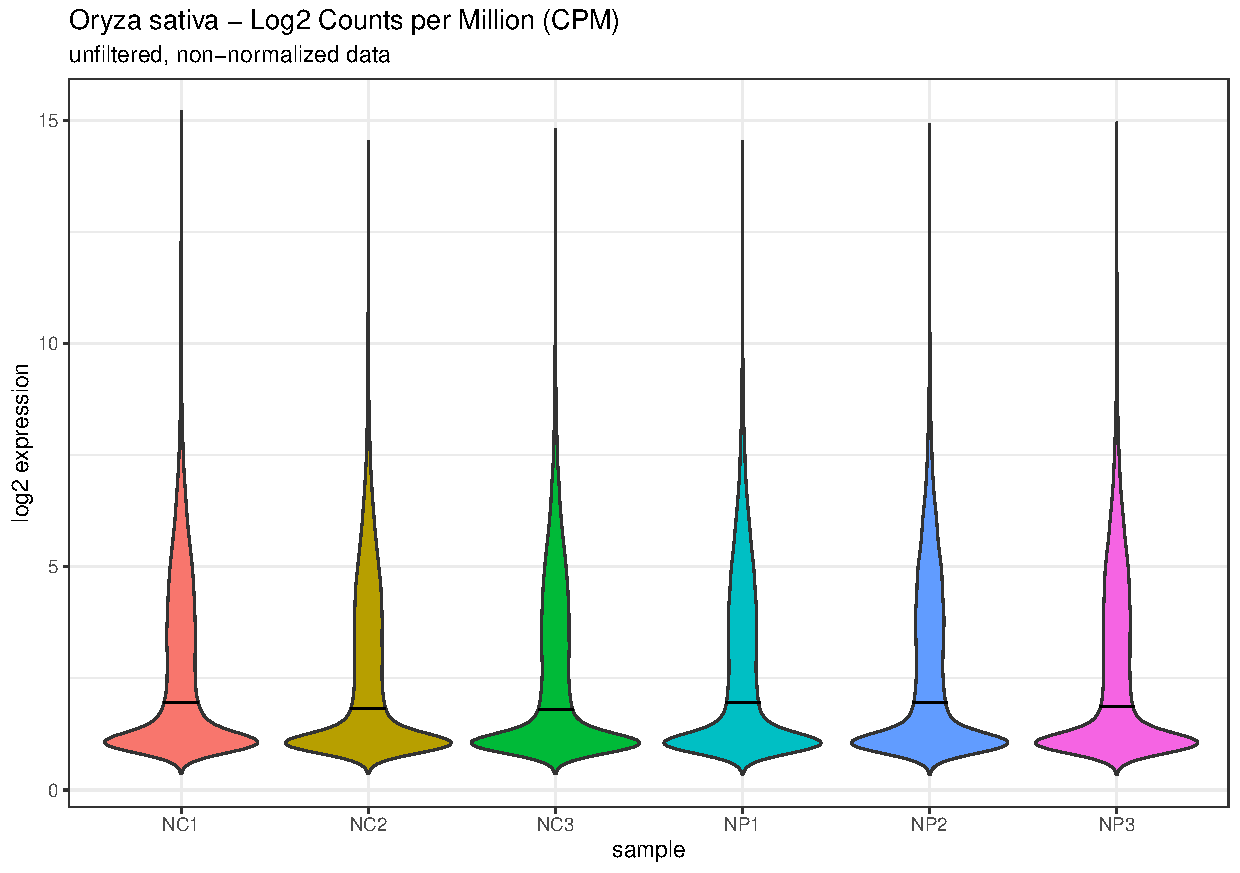
\includegraphics[width=\textwidth, height=3cm]{../../results/plots-and-tables/2.2-Log2CPM-unflt-notnorm-Oryza_sativa}
    \end{subfigure}
\end{figure}

In order to assess reasonable values for filtering the data, the number of genes with no reads at all (in none of the samples) and conversely the number of genes with CPMs \(\ge 1\) in at least 1, 2, 3, \dots\ of the samples were computed. Table \ref{tab:ufltr_cpm_stats} summarizes the results.

\begin{table}[htbp]
    \begin{threeparttable}
        \caption[Number of genes with no reads, and number of genes with  CPMs \(\ge 1\)]{Number of genes with no reads at all, and conversely number of genes with CPMs \(\ge 1\) in at least n = 1, 2, 3, \dots\ of the samples}
        \label{tab:ufltr_cpm_stats}
        \setlength\tabcolsep{5pt}
        \begin{tabular}{l l l p{30pt} p{30pt} p{30pt} p{30pt} p{30pt} p{30pt}}
            \toprule
                             &                  &                     & \multicolumn{6}{l}{Genes with CPMs \(\ge 1\) in at least n samples} \\
            \textbf{Species} & \(\Sigma\) genes & \(\Sigma\) no reads & 1     & 2     & 3     & 4     & 5     & 6     \\
            \midrule
            O. nivara        & 36313            & 7115                & 21001 & 20355 & 19891 & 19302 & 18895 & 18481 \\
            O. sativa        & 37967            & 4699                & 23934 & 22510 & 21609 & 20592 & 19715 & 18656 \\
            \bottomrule
        \end{tabular}
    \end{threeparttable}
\end{table}

Filtering out genes with low reads (\(< 1\) CPM in at least half of the samples) resulted in the distribution of the log2(CPM) values shown in figure \ref{fig:2.3-Log2CPM-flt-notnorm}.

\begin{figure}[htbp]
    \caption[Log2(CPM) distribution of the filtered, non-normalized data]{Log2(CPM) distribution of the filtered (\(< 1\) CPM in at least half of the samples), non-normalized data}
    \label{fig:2.3-Log2CPM-flt-notnorm}
    \begin{subfigure}[t]{0.64\linewidth}
        \caption{O. nivara}
        \label{fig:2.3-Log2CPM-flt-notnorm-Oryza_nivara}
        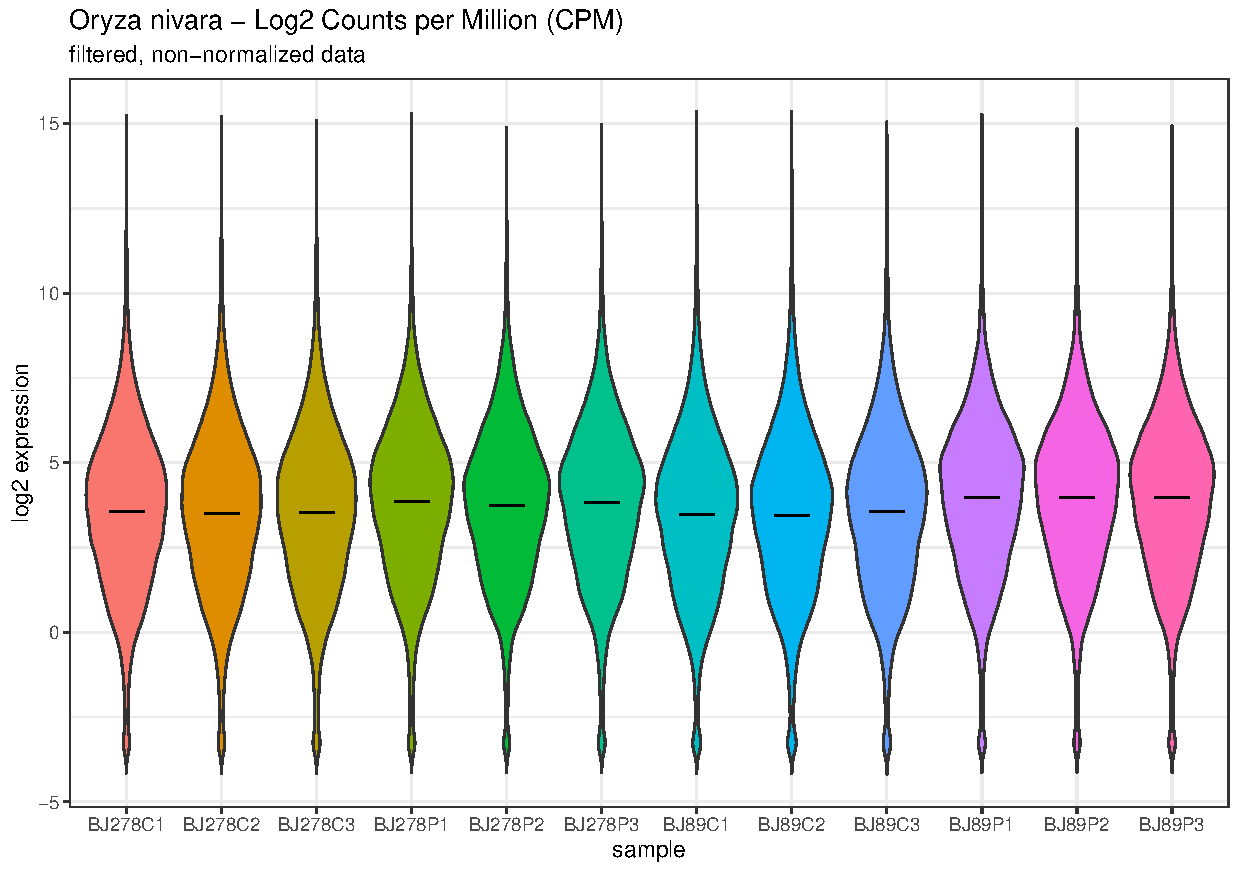
\includegraphics[width=\textwidth, height=3cm]{../../results/plots-and-tables/2.3-Log2CPM-flt-notnorm-Oryza_nivara}
    \end{subfigure}
    \begin{subfigure}[t]{0.32\linewidth}
        \caption{O. sativa}
        \label{fig:2.3-Log2CPM-flt-notnorm-Oryza_sativa}
        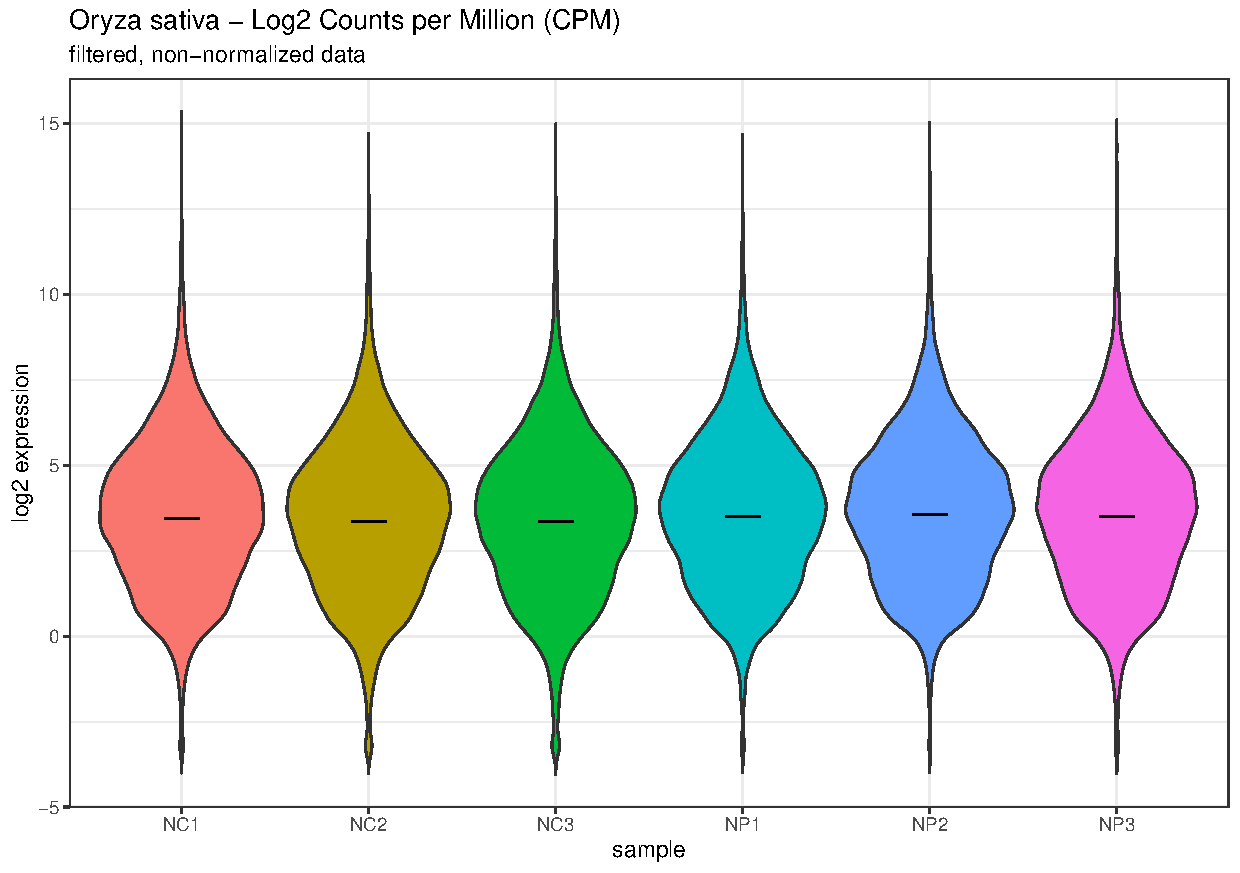
\includegraphics[width=\textwidth, height=3cm]{../../results/plots-and-tables/2.3-Log2CPM-flt-notnorm-Oryza_sativa}
    \end{subfigure}
\end{figure}

Finally, the filtered data was normalized using the \verb|edgeR| function \verb|calcNormFactors| which calculates scaling factors to convert raw library sizes into effective library sizes. Used normalization method: \verb|TMM|. The results of the normalization are shown in figure \ref{fig:2.4-Log2CPM-flt-norm}.

\begin{figure}[htbp]
    \caption{Log2(CPM) distribution of the filtered, normalized data}
    \label{fig:2.4-Log2CPM-flt-norm}
    \begin{subfigure}[t]{0.64\linewidth}
        \caption{O. nivara}
        \label{fig:2.4-Log2CPM-flt-norm-Oryza_nivara}
        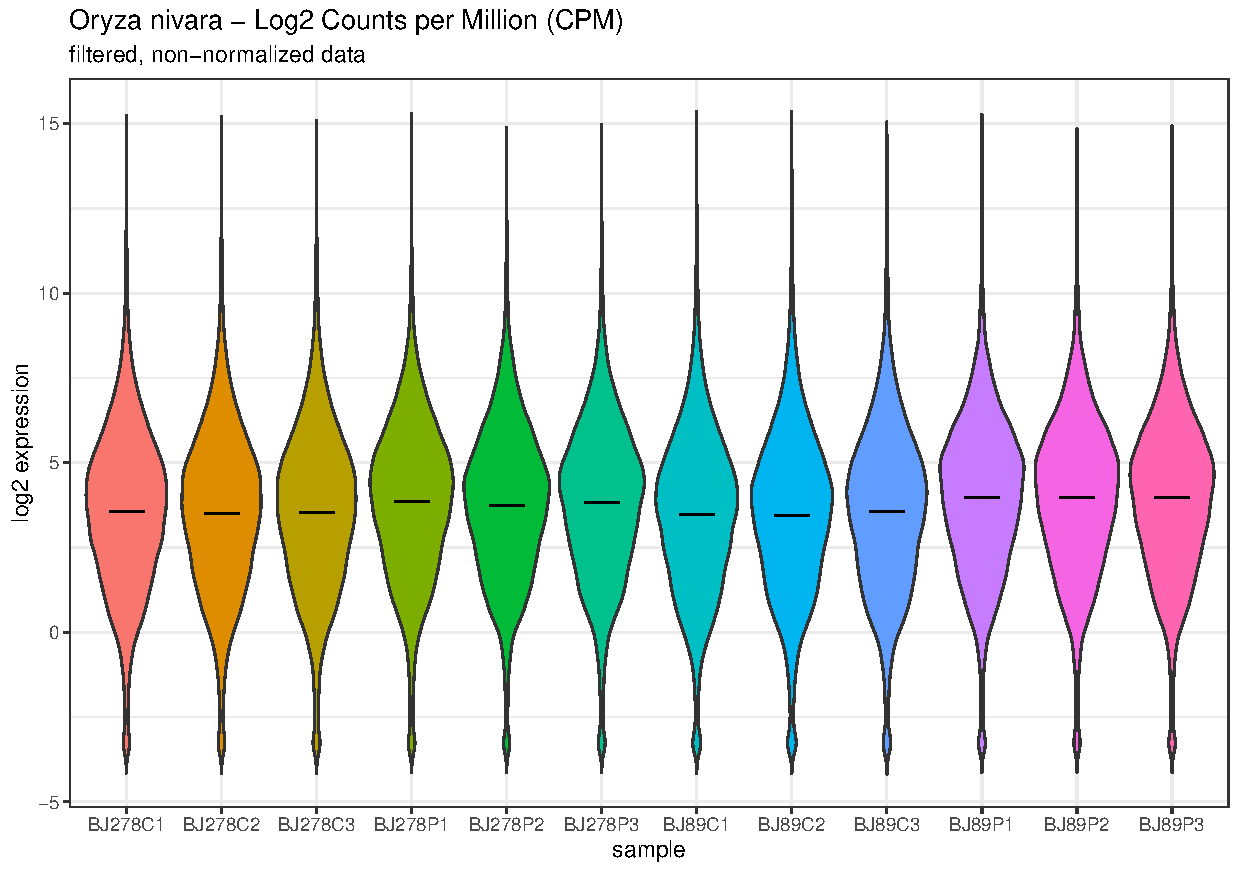
\includegraphics[width=\textwidth, height=3cm]{../../results/plots-and-tables/2.3-Log2CPM-flt-notnorm-Oryza_nivara}
    \end{subfigure}
    \begin{subfigure}[t]{0.32\linewidth}
        \caption{O. sativa}
        \label{fig:2.4-Log2CPM-flt-norm-Oryza_sativa}
        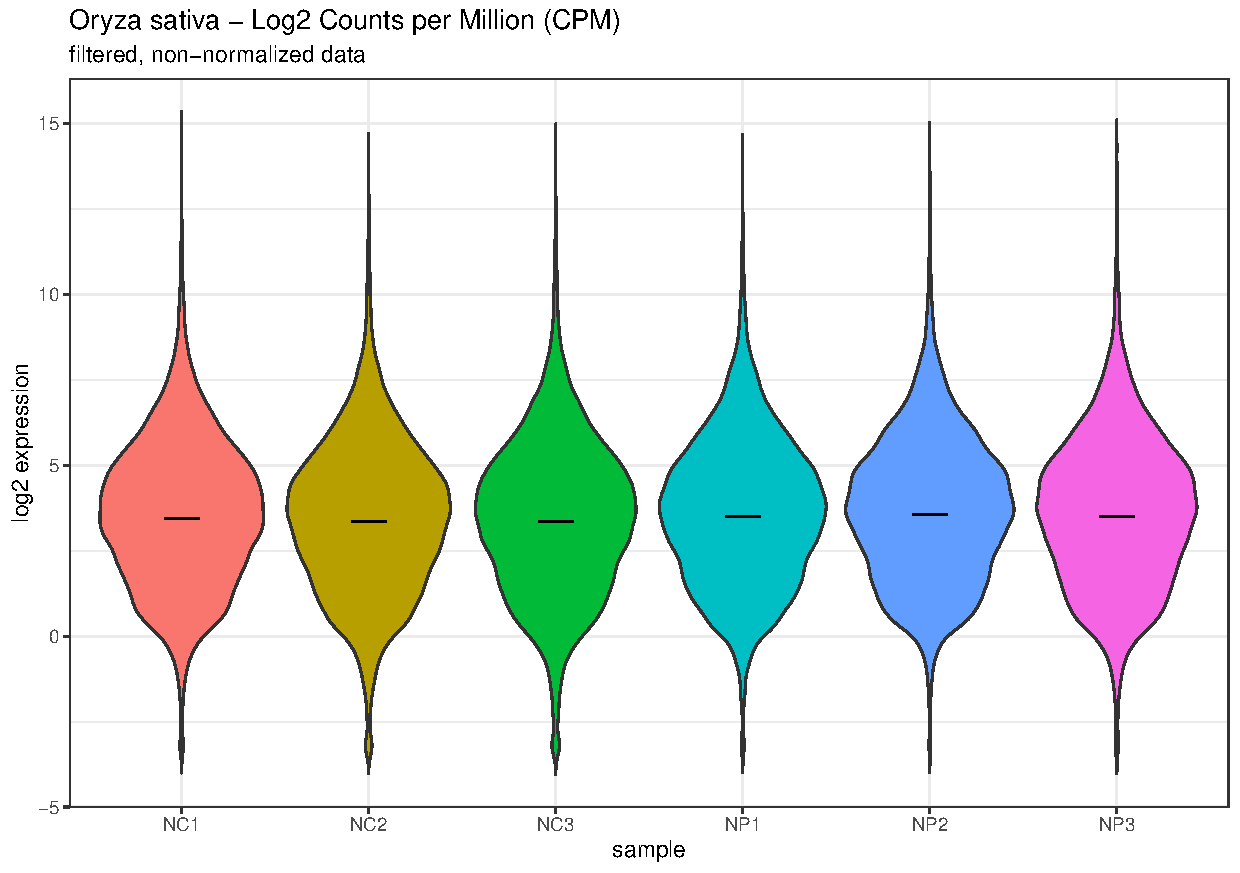
\includegraphics[width=\textwidth, height=3cm]{../../results/plots-and-tables/2.3-Log2CPM-flt-notnorm-Oryza_sativa}
    \end{subfigure}
\end{figure}

Figure \ref{fig:2.5-Log2CPM-Overview} provides an overview of the filtering and normalization results.

\begin{figure}[htbp]
    \caption{Log2(CPM) distribution of the filtered, normalized data in comparison with the non-normalized and the unfiltered data}
    \label{fig:2.5-Log2CPM-Overview}
    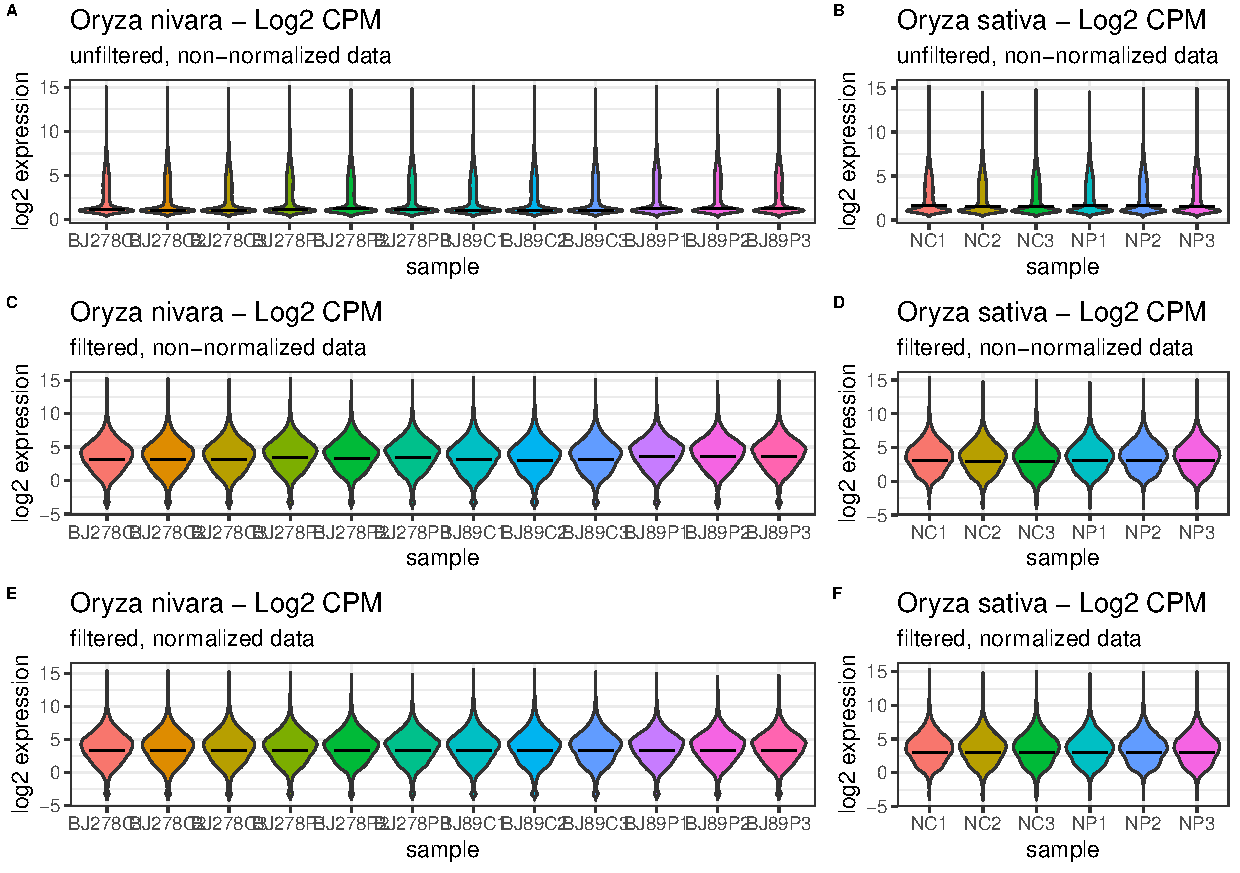
\includegraphics[width=\textwidth]{../../results/plots-and-tables/2.5-Log2CPM-Overview}
\end{figure}

\subsubsection{Hierarchical cluster analysis}

A hierarchical cluster analysis (HCA)\index{hierarchical cluster analysis (HCA)} was performed via the \verb|stats|\index{R!package!stats} function \verb|hclust| on the Euclidean distance matrix\index{hierarchical cluster analysis (HCA)!Euclidean distance matrix} of the log2(CPM) values. Used agglomeration method: \verb|method = complete|.

\subsubsection{Principal component analysis}

A principal component analysis (PCA)\index{principal component analysis (PCA)} of the filtered and normalized log2(CPM) values was performed via the \verb|stats|\index{R!package!stats} function \verb|prcomp|.

\subsubsection{Identification of differentially expressed genes}

In order to identify differentially expressed genes (DEGs)\index{differentially expressed genes (DEGs)}, design and contrast matrices were created using the \verb|stats|\index{R!package!stats} function \verb|model.matrix| and the \verb|limma|\index{R!package!limma} function \verb|makeContrasts|.

The design matrices were used to create linear model fits for each gene via the \verb|limma|\index{R!package!limma} functions \verb|voom| and \verb|lmFit|.

The linear model fits and the contrast matrices were used to calculate estimated coefficients and standard errors (contrasts) via the \verb|limma|\index{R!package!limma} function \verb|contrasts.fit|.

The contrasts were used to "calculate moderated t-statistics, moderated F-statistic, and log-odds of differential expression by empirical Bayes moderation of the standard errors towards a global value" (empirical Bayes statistics) via the \verb|limma|\index{R!package!limma} function \verb|eBayes| \autocite{R-limma}.

Finally, the empirical Bayes statistics were used to extract a table of the top-ranked genes via the \verb|limma|\index{R!package!limma} function \verb|topTable| (sorted by the \verb|LogFC|\index{LogFC}-values).

Venn diagrams of the DEGs (according to the calculated empirical Bayes statistics) were created via the \verb|gprofiler2|\index{R!package!gprofiler2} function \verb|decideTests| (with parameters \verb|method = "global"|, \verb|adjust.method = "BH"|, \verb|p.value = 0.01|, \verb|lfc = 7|) and the \verb|limma| function \verb|vennDiagram|.

See \autocite{limma2015} for details on the statistical foundations implemented by \verb|limma|\index{R!package!limma}.

\subsection{Functional enrichment analysis}

A functional enrichment analysis\index{functional enrichment analysis} of the 100 "top-ranked" genes was performed via the \verb|gprofiler2|\index{R!package!gprofiler2} function \verb|gost| (with \verb|correction_method = "fdr"| \autocite{R-gprofiler2}.